%----------------------------------------------------------------------------------------
%	PACKAGES AND OTHER DOCUMENT CONFIGURATIONS
%----------------------------------------------------------------------------------------

\documentclass[paper=a4, fontsize=11pt]{scrartcl} % A4 paper and 11pt font size

% ---- Entrada y salida de texto -----

\usepackage[T1]{fontenc} % Use 8-bit encoding that has 256 glyphs
\usepackage[utf8]{inputenc}
%\usepackage{fourier} % Use the Adobe Utopia font for the document - comment this line to return to the LaTeX default

% ---- Idioma --------

\usepackage[spanish, es-tabla]{babel} % Selecciona el español para palabras introducidas automáticamente, p.ej. "septiembre" en la fecha y especifica que se use la palabra Tabla en vez de Cuadro

% ---- Otros paquetes ----
\usepackage{csquotes} %Para permitir el uso de comillas Quotes https://tex.stackexchange.com/questions/36812/isnt-there-any-other-way-of-doing-double-quotes-in-latex-besides
\usepackage[hyphens]{url} % ,href} %para incluir URLs e hipervínculos dentro del texto (aunque hay que instalar href)
\usepackage{hyperref}
\usepackage{color}
\usepackage{graphics,graphicx, floatrow} %para incluir imágenes y notas en las imágenes
\usepackage{graphics,graphicx, float} %para incluir imágenes y colocarlas

\graphicspath {{./img/}}

\usepackage{listings}  %para introducir comandos

\lstdefinestyle{mybash}
{basicstyle=\ttfamily,
  showstringspaces=false,
  commentstyle=\color{red},
  keywordstyle=\color{blue},
  language=bash,
  alsoletter=/,
  basicstyle=\footnotesize,
  numbers=left,
  stepnumber=1,
  showstringspaces=false,
  tabsize=1,
  breaklines=true,
  breakatwhitespace=false,
}
\lstdefinestyle{mysql}
{basicstyle=\ttfamily,
  showstringspaces=false,
  commentstyle=\color{red},
  keywordstyle=\color{blue},
  language=sql,
  basicstyle=\footnotesize,
  numbers=left,
  stepnumber=1,
  showstringspaces=false,
  tabsize=1,
  breaklines=true,
  breakatwhitespace=false,
}


% Para hacer tablas comlejas
%\usepackage{multirow}
%\usepackage{threeparttable}

%\usepackage{sectsty} % Allows customizing section commands
%\allsectionsfont{\centering \normalfont\scshape} % Make all sections centered, the default font and small caps

\usepackage{fancyhdr} % Custom headers and footers
\pagestyle{fancyplain} % Makes all pages in the document conform to the custom headers and footers
\fancyhead{} % No page header - if you want one, create it in the same way as the footers below
\fancyfoot[L]{} % Empty left footer
\fancyfoot[C]{} % Empty center footer
\fancyfoot[R]{\thepage} % Page numbering for right footer
\renewcommand{\headrulewidth}{0pt} % Remove header underlines
\renewcommand{\footrulewidth}{0pt} % Remove footer underlines
\setlength{\headheight}{13.6pt} % Customize the height of the header

\setlength\parindent{0pt} % Removes all indentation from paragraphs - comment this line for an assignment with lots of text

\newcommand{\horrule}[1]{\rule{\linewidth}{#1}} % Create horizontal rule command with 1 argument of height


%----------------------------------------------------------------------------------------
%	TÍTULO Y DATOS DEL ALUMNO
%----------------------------------------------------------------------------------------
\graphicspath{ {img/} }

\title{
\normalfont \normalsize

\includegraphics[width=6cm,height=6cm]{logo}\\
\textsc{\textbf{Bootcamp Especialidad GNU/Linux (2023)}} \\ [25pt] % Your university, school and/or department name(s)
\horrule{0.5pt} \\[0.4cm] % Thin top horizontal rule
\huge Lab 07 - Configuración de copias de seguridad en bases de datos \\ % The assignment title
\horrule{2pt} \\[0.5cm] % Thick bottom horizontal rule
}


%https://es.overleaf.com/learn/latex/Inserting_Images
%Ruta relativa de   imagenes

\author{Pedro Antonio Mayorgas Parejo} % Nombre y apellidos

\date{\normalsize\today} % Incluye la fecha actual

%----------------------------------------------------------------------------------------
% DOCUMENTO
%----------------------------------------------------------------------------------------

\begin{document}

\maketitle % Muestra el Título

\newpage %inserta un salto de página

\tableofcontents % para generar el índice de contenidos

\newpage

%----------------------------------------------------------------------------------------
%	Cuestión 1
%----------------------------------------------------------------------------------------

\section{Instalación de Sistema Gestor de Base de Datos}

Para la instalación del SGBD, debemos en ejecutar el siguiente comando en una distribución Debian GNU/Linux.

\begin{lstlisting}[style=mybash]
sudo apt install mariadb-server
\end{lstlisting}

\begin{figure}[H]
	\centering
	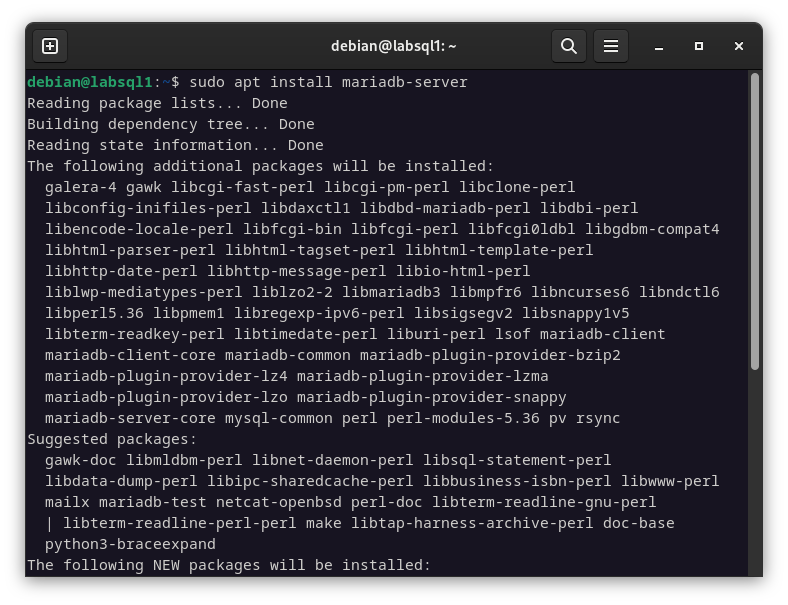
\includegraphics[scale=0.30]{00}
	\caption{Instalación de MariaDB server.}
\end{figure}


A continuación ejecutamos el siguiente comando, para asegurar el SGBD. En realidad no es un comando, es un script especial que permite el aumento de la seguridad de las bases de datos de MariaDB o MySQL.

\begin{lstlisting}[style=mybash]
sudo mysql_secure_installation
\end{lstlisting}

\begin{figure}[H]
	\centering
	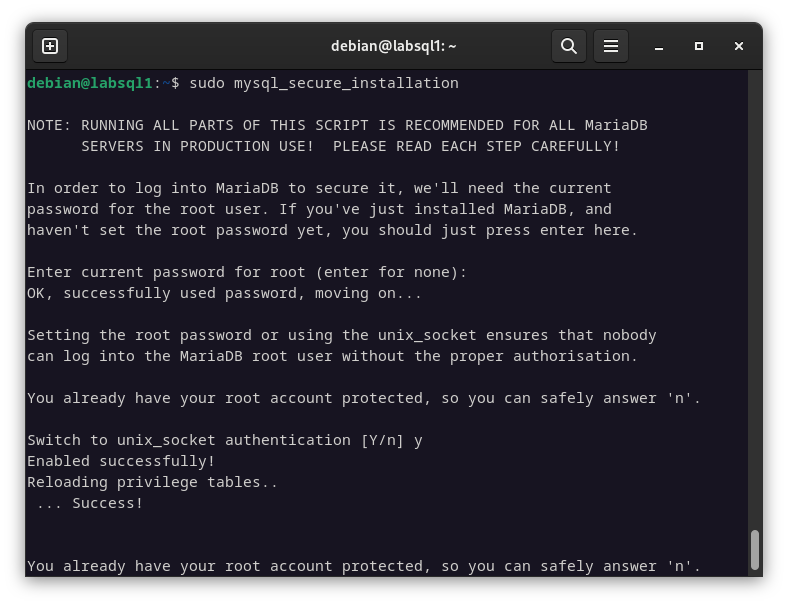
\includegraphics[scale=0.30]{01}
	\caption{Ejecución de mysql\_secure\_installation.}
\end{figure}

En la captura anterior, permitimos la conexión del tipo solo con Sockets, es decir, que 

\begin{figure}[H]
	\centering
	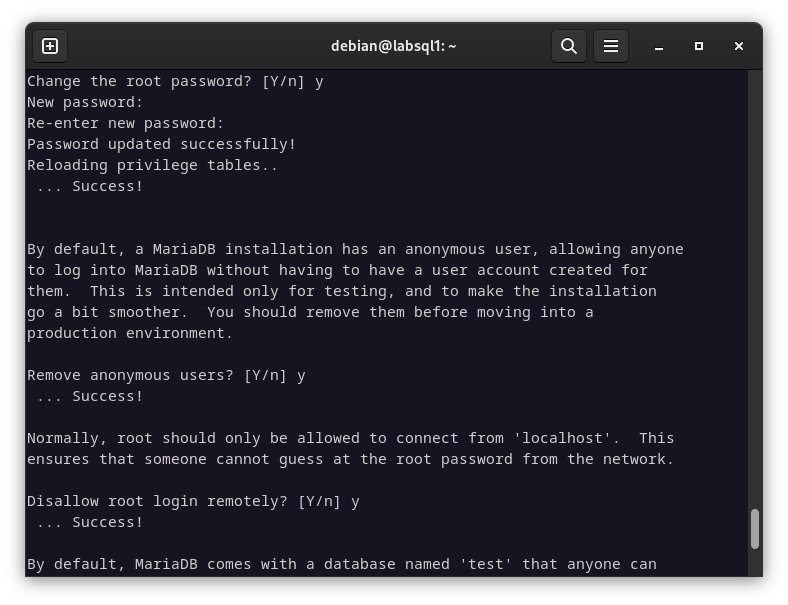
\includegraphics[scale=0.30]{02}
	\caption{Ejecución de mysql\_secure\_installation - Parte de Usuarios y login.}
\end{figure}

En la captura anterior, eliminamos las tablas privilegiadas, eliminamos los usuarios anónimos que permiten que sean autenticados hacia el SGBD sin tener un usuario en concreto creado por el administrador de bases de datos. Por último bloqueamos la autenticación de root de manera remota.

\begin{figure}[H]
	\centering
	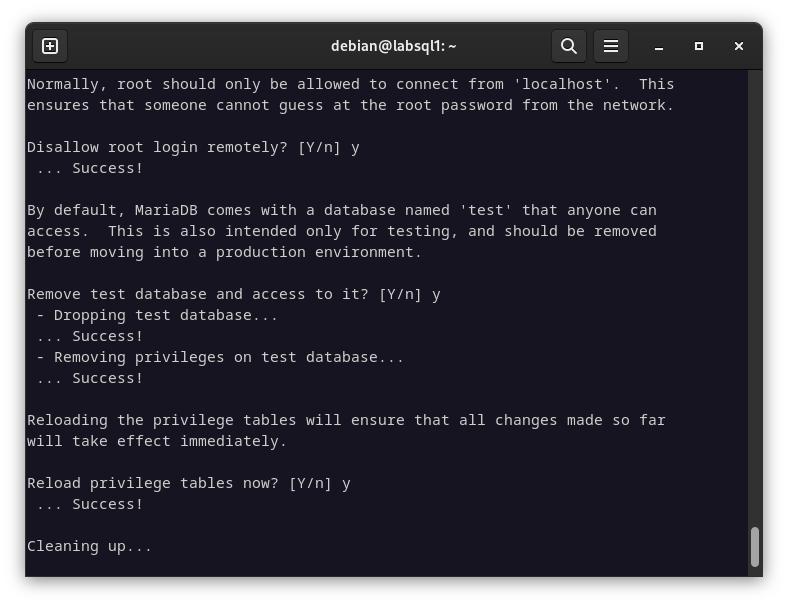
\includegraphics[scale=0.30]{03}
	\caption{Ejecución de mysql\_secure\_installation - Eliminación de base de datos de test y su acceso.}
\end{figure}

Ahora tenemos que borrar las bases de datos de test, así como recargar los permisos de acceso.

\newpage
\section{Datos de la base de datos}

Ahora los datos de la base de datos que son introducidos, de manera general son los siguientes:

\begin{figure}[H]
	\centering
	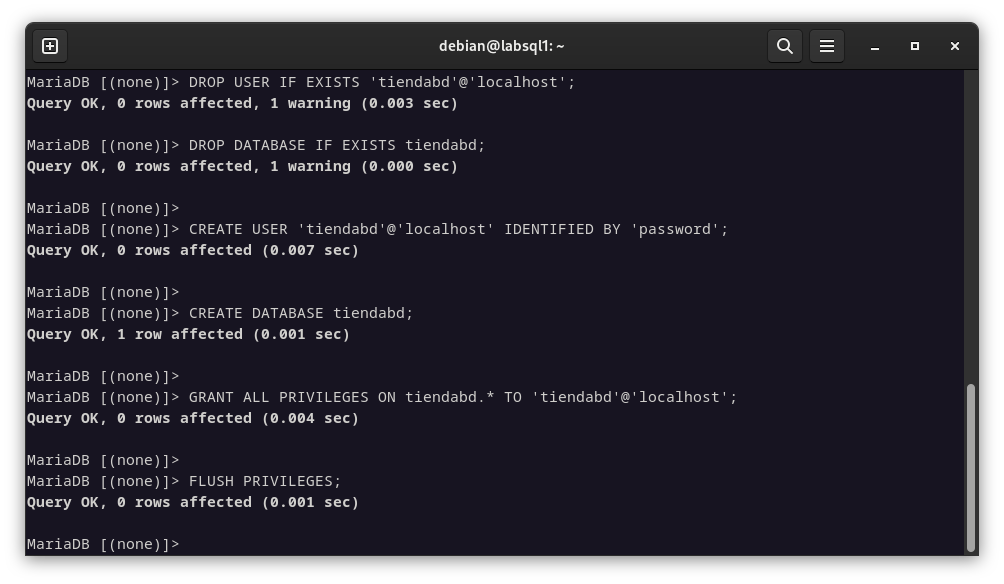
\includegraphics[scale=0.30]{04}
	\caption{Ejecución de SQL - Creando usuario, base de datos y permisos.}
\end{figure}

\begin{figure}[H]
	\centering
	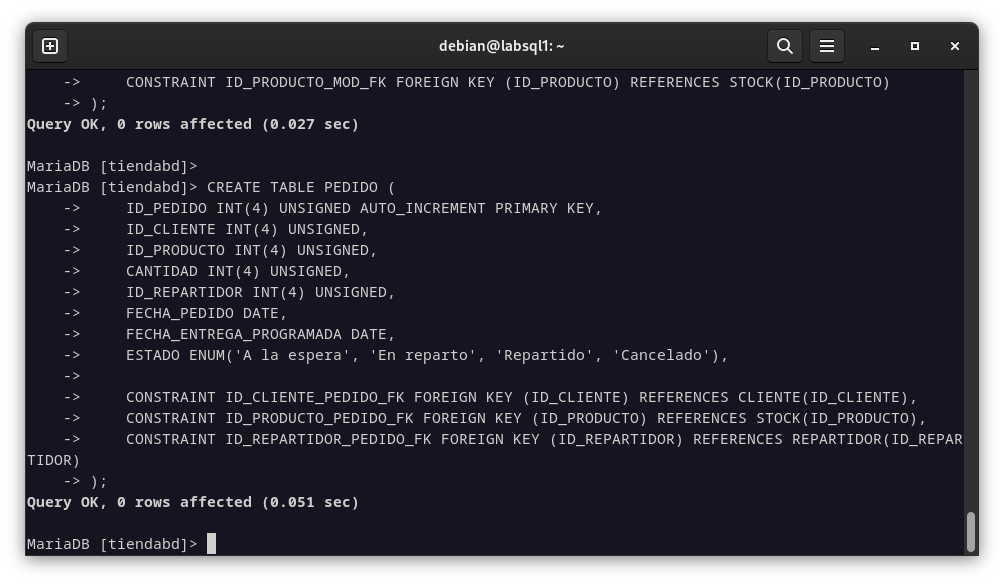
\includegraphics[scale=0.30]{05}
	\caption{Ejecución de SQL - Creando tablas dentro de la base de datos.}
\end{figure}

\begin{figure}[H]
	\centering
	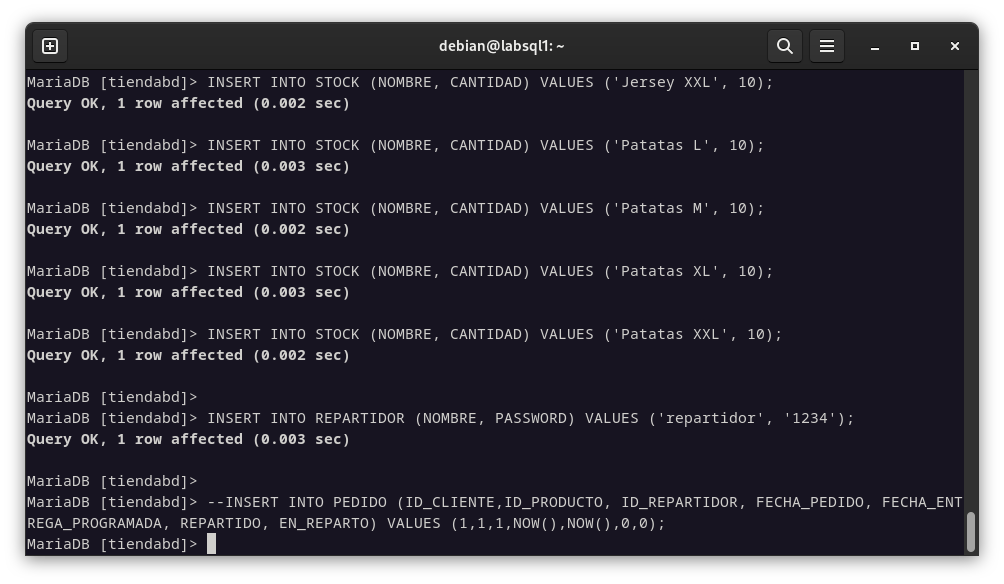
\includegraphics[scale=0.30]{06}
	\caption{Ejecución de SQL - Insertando datos en tablas dentro de la base de datos..}
\end{figure}

\newpage
\section{Script de Bash para CRON}

El script realiza las copias de seguridad periódicas con mysqldump, con algunos parámetros ajustables que son explicados dentro del mismo, en resumen se permite afinar el dump según los parámetros que exiga el administrador. Así como indicar a través de variables los datos de la base de datos y su usuario. 
\vspace{5mm}

El usuario debe tener los permisos indicados dentro del script, de lo contrario no podrá hacer el dump.

\lstinputlisting[style=mybash]{scripts/script01.sh}

\newpage
Luego el siguiente script, funciona como archivador, para que no se generen infinitos ficheros .sql, permitiendo que se puedan almacenar por cada día todos los .sql generados y poder limpiar la carpeta para el día siguiente.

\lstinputlisting[style=mybash]{scripts/script02.sh}


Ahora movemos los scripts a un directorio más adecuado para la ejecución por parte de cron.

\begin{lstlisting}[style=mybash]
cp script01.sh /usr/local/sbin
cp script02.sh /usr/local/sbin
sudo apt install cron
# EDITAMOS EL CRONTAB
sudo crontab -e
\end{lstlisting}

\begin{figure}[H]
	\centering
	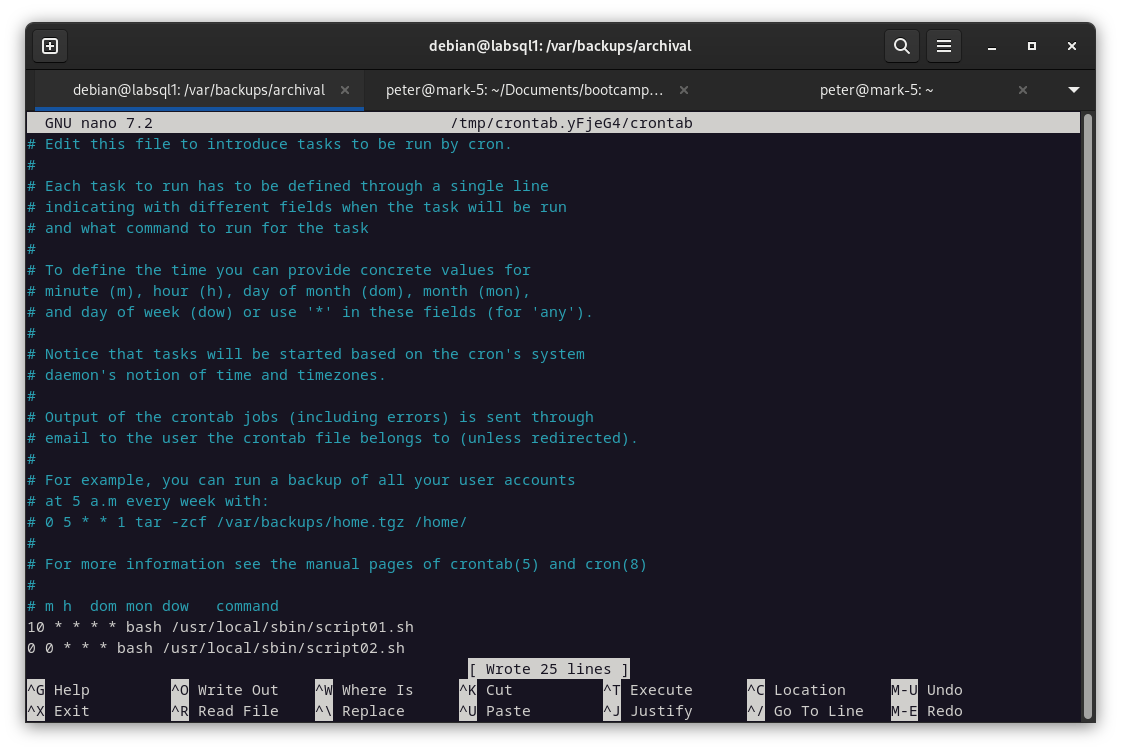
\includegraphics[scale=0.30]{07}
	\caption{Crontab editado}
\end{figure}

\begin{figure}[H]
	\centering
	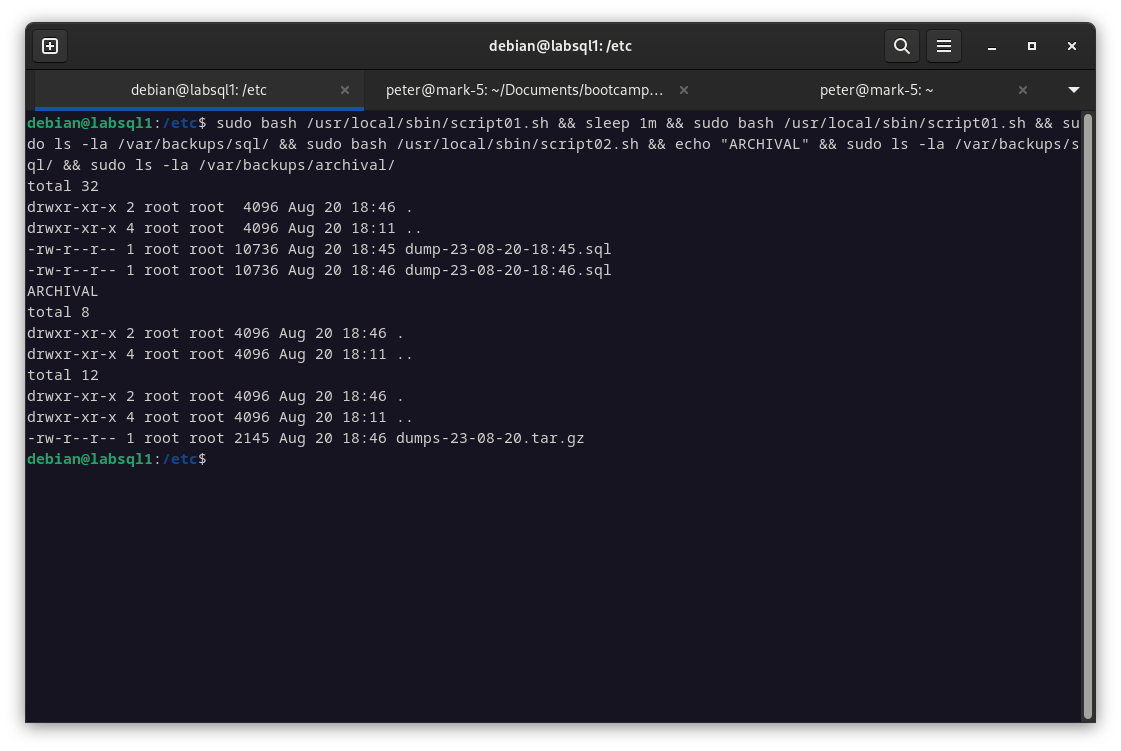
\includegraphics[scale=0.30]{08}
	\caption{Resultado si ejecutamos los scripts}
\end{figure}

% \vspace{5mm}


% \begin{lstlisting}[style=mybash]
%     # Para una base de datos concreta
%     mysqldump --user=tiendabd --password=password --databases tiendabd --add-drop-database --add-drop-table [--replace] --host=127.0.0.1 --result-file=dump.sql
% \end{lstlisting}



%\begin{figure}[H]
%	\centering
%	\includegraphics[scale=0.30]{cuestion_1_1}
%	\caption{Se puede ver que al no haber un fallo grave, el sistema lo nota como que sigue funcionando pero en un estado degradado.}
%\end{figure}

%\newpage

%Se pueden hacer include en latex
%\newpage

\section{Section}

\subsection{Subseccion}

\subsubsection{Subseccion}



%-------Bibliografia-----------------------------

%\newpage
\section{Bibliografía}

% Ejemplo
\footnote{Administración de mdadm - Por Red Hat}
\textcolor{blue}{\url{https://access.redhat.com/documentation/en-us/red_hat_enterprise_linux/8/html/managing_storage_devices/managing-raid_managing-storage-devices#monitoring-raid_managing-raid}}



\end{document}
